\documentclass{article}

\title{Part 1: The Basics of Production\\Chapters 1 to 2}
\author{Vladimir Feinberg}

% latex math commands
% Vladimir Feinberg
% \vx notation for vectors from Goodfellow
% https://github.com/goodfeli/dlbook_exercises

% alphabet templates
% abcdefghijklmnopqrstuvwxyz
% ABCDEFGHIJKLMNOPQRSTUVWXYZ

% fonts, math, and layout commands
\usepackage{fullpage}


\usepackage{setspace} % for \onehalfspacing and \singlespacing macros
\onehalfspacing 

\usepackage{etoolbox}
\AtBeginEnvironment{quote}{\singlespacing\small}

\usepackage{bbm}
\usepackage{enumerate}
\usepackage{amsmath}
\usepackage{amsthm}
\usepackage{amssymb}
\usepackage{amsfonts}
\usepackage{mathrsfs}
\usepackage{mathtools}
\usepackage[all]{xy}

% include graphics with \includegraphics
\usepackage{graphicx}
\usepackage{caption}

% \nicefrac{x}{y} gives a diagonal fraction bar x/y
\usepackage{nicefrac}

% \nurl{<url>}{link name} renders a blue underlined link
\usepackage[hidelinks]{hyperref}
\usepackage{xcolor}
\usepackage{url}
\newcommand{\nurl}[2]{\href{ #1 }{\color{blue}\underline{#2}}}

% brackets, norms, cardinalities
\newcommand{\pa}[1]{ \left({#1}\right) }
\newcommand{\ha}[1]{ \left[{#1}\right] }
\newcommand{\ca}[1]{ \left\{{#1}\right\} }
\newcommand{\inner}[1]{\left\langle #1 \right\rangle}
\newcommand{\innercpy}[1]{\inner{ #1, #1 }}
\newcommand{\norm}[1]{\left\lVert #1 \right\rVert}
\newcommand{\card}[1]{\left\lvert{#1}\right\rvert}
\newcommand{\abs}[1]{\card{#1}}

% math vectors
\newcommand{\va}{\textbf{a}}
\newcommand{\vb}{\textbf{b}}
\newcommand{\vc}{\textbf{c}}
\newcommand{\vd}{\textbf{d}}
\newcommand{\ve}{\textbf{e}}
\newcommand{\vf}{\textbf{f}}
\newcommand{\vg}{\textbf{g}}
\newcommand{\vh}{\textbf{h}}
\newcommand{\vi}{\textbf{i}}
\newcommand{\vj}{\textbf{j}}
\newcommand{\vk}{\textbf{k}}
\newcommand{\vl}{\textbf{l}}
\newcommand{\vm}{\textbf{m}}
\newcommand{\vn}{\textbf{n}}
\newcommand{\vo}{\textbf{o}}
\newcommand{\vp}{\textbf{p}}
\newcommand{\vq}{\textbf{q}}
\newcommand{\vr}{\textbf{r}}
\newcommand{\vs}{\textbf{s}}
\newcommand{\vt}{\textbf{t}}
\newcommand{\vu}{\textbf{u}}
\newcommand{\vv}{\textbf{v}}
\newcommand{\vw}{\textbf{w}}
\newcommand{\vx}{\textbf{x}}
\newcommand{\vy}{\textbf{y}}
\newcommand{\vz}{\textbf{z}}
\newcommand{\vzero}{\textbf{0}}
\newcommand{\vone}{\textbf{1}} 
\newcommand{\valpha}{{\boldsymbol\alpha}}
\newcommand{\vepsilon}{{\boldsymbol\epsilon}}
\newcommand{\veta}{{\boldsymbol\eta}}
\newcommand{\vsigma}{ {\boldsymbol\sigma}}
\newcommand{\vtheta}{ {\boldsymbol\theta}}
\newcommand{\vdelta}{ {\boldsymbol\delta}}
\newcommand{\vlambda}{ {\boldsymbol\lambda}}
\newcommand{\vmu}{ {\boldsymbol\mu}}
\newcommand{\vvartheta}{ {\boldsymbol\vartheta}}
\newcommand{\vbeta}{ {\boldsymbol\beta}}
\newcommand{\vphi}{ {\boldsymbol\phi}}


% math function arrows, misc binary math ops
\newcommand{\bij}{\leftrightarrow}
\newcommand{\inj}{\rightarrowtail}
\newcommand{\sur}{\twoheadedrightarrow}
\newcommand{\eqd}{\mathrel{\overset{\Delta}{=}}}

% common math sets
\newcommand{\Z}{\mathbb{Z}}
\newcommand{\R}{\mathbb{R}}
\newcommand{\C}{\mathbb{C}}
\newcommand{\N}{\mathbb{N}}
\newcommand{\Q}{\mathbb{Q}}
\newcommand{\F}{\mathbb{F}}
\newcommand{\T}{\mathbb{T}}

% limits
\def\sumn{\sum_{n=0}^\infty}
\def\limn{\lim_{n\rightarrow\infty}}
\def\prodn{\prod_{n=0}^\infty}

% mathcal
\newcommand{\mcA}{\mathcal{A}}
\newcommand{\mcB}{\mathcal{B}}
\newcommand{\mcC}{\mathcal{C}}
\newcommand{\mcD}{\mathcal{D}}
\newcommand{\mcE}{\mathcal{E}}
\newcommand{\mcF}{\mathcal{F}}
\newcommand{\mcG}{\mathcal{G}}
\newcommand{\mcH}{\mathcal{H}}
\newcommand{\mcI}{\mathcal{I}}
\newcommand{\mcJ}{\mathcal{J}}
\newcommand{\mcK}{\mathcal{K}}
\newcommand{\mcL}{\mathcal{L}}
\newcommand{\mcM}{\mathcal{M}}
\newcommand{\mcN}{\mathcal{N}}
\newcommand{\mcO}{\mathcal{O}}
\newcommand{\mcP}{\mathcal{P}}
\newcommand{\mcQ}{\mathcal{Q}}
\newcommand{\mcR}{\mathcal{R}}
\newcommand{\mcS}{\mathcal{S}}
\newcommand{\mcT}{\mathcal{T}}
\newcommand{\mcU}{\mathcal{U}}
\newcommand{\mcV}{\mathcal{V}}
\newcommand{\mcW}{\mathcal{W}}
\newcommand{\mcX}{\mathcal{X}}
\newcommand{\mcY}{\mathcal{Y}}
\newcommand{\mcZ}{\mathcal{Z}}

% measure theory, distributions
\newcommand{\indicator}{\mathbbm{1}}
\DeclareMathOperator{\Laplace}{Laplace}
\DeclareMathOperator{\soft}{soft}
\DeclareMathOperator{\hard}{hard}
\DeclareMathOperator{\clo}{clo}
\DeclareMathOperator{\Poisson}{Poisson}
\DeclareMathOperator{\Exponential}{Exponential}
\DeclareMathOperator{\Multinomial}{Multinomial}
\DeclareMathOperator{\Bernoulli}{Bernoulli}
\DeclareMathOperator{\Categorical}{Categorical}
\DeclareMathOperator{\Uniform}{Uniform}
\DeclareMathOperator{\Binomial}{Binomial}
\DeclareMathOperator{\Hypergeometric}{Hypergeometric}
\DeclareMathOperator{\GammaDist}{Gamma}
\DeclareMathOperator{\NegativeBinomial}{NegativeBinomial}
\DeclareMathOperator\mathProb{\mathbb{P}}
\DeclareMathOperator\sub{sub}
\renewcommand{\d}[1]{\mathop{\mathrm{d} #1 }}
\DeclarePairedDelimiterX{\infdivx}[2]{(}{)}{ #1\;\delimsize\|\;#2 }
\newcommand{\dkl}[2]{\mathop{D_\text{KL}}\infdivx{#1}{#2}}
\newcommand{\sg}{\mathop{\mathrm{SG}}}
\newcommand{\se}{\mathop{\mathrm{SE}}}

% distributions
\makeatletter
\newcommand{\distas}[1]{\mathbin{\overset{#1}{\kern\z@\sim}}}%
\makeatother
\newcommand{\disteq}{\overset{d}{=}}
\newcommand{\distiid}{\distas{\text{iid}}}
\newcommand\independent{\protect\mathpalette{\protect\independenT}{\perp}}
\def\independenT#1#2{\mathrel{\rlap{$#1#2$}\mkern2mu{#1#2}}}
\newcommand{\convdist}{\mathbin{\overset{\text{d}}{\longrightarrow}}}
\newcommand{\convas}{\mathbin{\overset{\text{as}}{\longrightarrow}}}
\newcommand{\convpb}{\mathbin{\overset{\text{pb}}{\longrightarrow}}}

\renewcommand{\P}{\mathProb} % need to overwrite stupid paragraph symbol
\DeclareMathOperator\mathExp{\mathbb{E}}
\DeclareMathOperator*\mathExpUnder{\mathbb{E}}
\newcommand{\E}{\mathExp}

\newcommand{\sa}{{$\sigma$-algebra}}
\newcommand{\OR}{{\overline{\R}}}
\newcommand{\OX}{{\overline{X}}}
\DeclareMathOperator{\power}{{\mathcal{P}}}
\DeclareMathOperator{\var}{var}
\DeclareMathOperator{\cov}{cov}

% \set{from set}{condition} with set-builder notation
% conditional expectation is analogous
\newcommand{\set}[2]{ \left\{ #1 \,\middle|\, #2 \right\} }
\newcommand{\CE}[2]{ \mathExp\left[ #1 \,\middle|\, #2 \right] }
\newcommand{\CP}[2]{ \mathProb\left\{ #1 \,\middle|\, #2 \right\} }

% linear-algebra related
\newcommand{\rip}{\operatorname{RIP}}
\DeclareMathOperator{\svd}{svd}
\newcommand{\frob}[1]{\norm{#1}_{\mathrm{F}}}
\newcommand{\mat}[1]{\begin{pmatrix} #1 \end{pmatrix}}
\newcommand{\detmat}[1]{\begin{vmatrix} #1 \end{vmatrix}}
\DeclareMathOperator{\spanb}{span}
\DeclareMathOperator{\conv}{conv} % convex hull
\DeclareMathOperator{\cone}{cone}
\DeclareMathOperator{\vectorize}{vec}
\DeclareMathOperator{\matricize}{mat}
\DeclareMathOperator{\adj}{adj}
\DeclareMathOperator{\diag}{diag}
\DeclareMathOperator{\tr}{tr}
\DeclareMathOperator{\rank}{rank}
\DeclareMathOperator*{\argmin}{argmin}
\DeclareMathOperator*{\argmax}{argmax}
\DeclareMathOperator*{\proj}{proj}

% complex analysis
\DeclareMathOperator{\MyRe}{Re}
\DeclareMathOperator{\MyIm}{Im}
\DeclareMathOperator{\image}{image}
\DeclareMathOperator{\supp}{supp}

% typical numerical operators
\DeclareMathOperator{\sgn}{sgn}

% graphs
\DeclareMathOperator{\diam}{diam}

% constants
\renewcommand{\d}[1]{\mathop{\mathrm{d} #1 }}
\newcommand{\e}{\mathrm{e}}
\renewcommand{\i}{\imath}

% \bigtimes: large indexed cross product
\makeatletter
\DeclareFontFamily{U}  {MnSymbolF}{}
\DeclareSymbolFont{symbolsMN}{U}{MnSymbolF}{m}{n}
\SetSymbolFont{symbolsMN}{bold}{U}{MnSymbolF}{b}{n}
\DeclareFontShape{U}{MnSymbolF}{m}{n}{
    <-6>  MnSymbolF5
   <6-7>  MnSymbolF6
   <7-8>  MnSymbolF7
   <8-9>  MnSymbolF8
   <9-10> MnSymbolF9
  <10-12> MnSymbolF10
  <12->   MnSymbolF12}{}
\DeclareFontShape{U}{MnSymbolF}{b}{n}{
    <-6>  MnSymbolF-Bold5
   <6-7>  MnSymbolF-Bold6
   <7-8>  MnSymbolF-Bold7
   <8-9>  MnSymbolF-Bold8
   <9-10> MnSymbolF-Bold9
  <10-12> MnSymbolF-Bold10
  <12->   MnSymbolF-Bold12}{}
\DeclareMathSymbol{\tbigtimes}{\mathop}{symbolsMN}{2}
\newcommand*{\bigtimes}{%
  \DOTSB
  \tbigtimes
  \slimits@ 
}
\makeatother

% category theory arguments
% See https://tex.stackexchange.com/questions/356873
\newcommand{\catfst}{{-}}
\newcommand{\catsnd}{{=}}
\newcommand{\cattrd}{{\equiv}}
\DeclareMathOperator{\Id}{Id}
\newcommand{\opcat}[1]{{#1}^{\text{op}}}
\DeclareMathOperator{\Hom}{hom}
\DeclareMathOperator{\Ob}{ob}
\DeclareMathOperator{\El}{el}
\DeclareMathOperator{\colim}{colim}
\DeclareMathOperator{\Sym}{Sym}
% restriction of a function to a domain
\newcommand\restr[2]{{% we make the whole thing an ordinary symbol
  \left.\kern-\nulldelimiterspace % automatically resize the bar with \right
  #1 % the function
  \vphantom{\big|} % pretend it's a little taller at normal size
  \right|_{#2} % this is the delimiter
  }}
\usepackage[all]{xy}


\begin{document}

\maketitle

Notes on Chapters 1 to 2 of Andy Grove's \textit{High Output Management} \cite{highoutput}.

Note that the sections are structured according to topics, not the chapters themselves

\section{Creating Production Requirements}

Work backwards from what the market needs. What do customers desire?

\begin{enumerate}
\item Timely delivery
\item High quality
\item Low cost
\end{enumerate}

Then the question is, how do you trade off each of the above? At Intel, the trade-off seemed to be

\begin{align*} 
  \min \,\,\,& \texttt{cost}\\
  \text{s.t.}\,\,\, & \texttt{quality}\ge \text{some acceptable threshold} \\
 & \texttt{delivery time}\le \text{sufficiently timely}
\end{align*}

But how should you set up the optimization problem in the context of your business? Andy does not answer this question for you. This is usually implied by your business model. For instance, for Amazon prime, delivery time is much more important, so Bezos might be interested in minimizing delivery time while keeping costs smaller than competitor's and quality at least as good as theirs.

Thus, the question of determining this aspect of your business model could in part be answered by considering the following.
\begin{enumerate}
\item Profile your customer to see what they care about more. For instance, in some industries, like e-commerce, cost is actually not as important as fast delivery turnaround (maybe, just guessing).
\item It just comes from the industry, market, and your business model or unique approach. This is what makes your business special: it's your business model
\end{enumerate}

\section{Production planning}

The key insight is to \textit{consider planning tasks with critical-path planning in the workflow DAG}. Work backwards from delivery time and requirements to construct the DAG of tasks to perform, and track the critical path progress over time.

Don’t forget to incorporate non-productive tasks into your planning.
\begin{enumerate}
\item Assembly
\item Testing
\item Inspection
\item Queue wait time in components that have limited capacity
\end{enumerate}

The above planning informs inventory purchases. For example, in a development environment, if your Travis Continuous Integration only handles 1 job at a time then you can’t merge in more than one PR every 30 minutes or however long your build time is. In turn, you should never bottleneck yourself on CI by buying more concurrent builds as you get more developers.

\section{Indicators}

Indicators enable appropriate and accurate forecasting for decision making, such as:

\begin{enumerate}
\item Sales forecasts
\item Manpower quantity and quality
\item Equipment status and output rate
\item Raw materials
\end{enumerate}

Taken on their own, indicators can result in a negative feedback loop. Paired indicators resolve Goodhart’s law-like bias from metrics. 

\begin{itemize}
\item For instance, suppose you’re measuring custodial staff by square feet cleaned alone. This may cause rooms to be poorly cleaned. By adding a complementary indicator, like the number of reports of unclean rooms, you can properly account for quality.
\item Analogously, if you only record the number of shortages, then you may over-supply your inventory to avoid shortages. But if you also record end-of-day remaining inventory then you know not to over-invest.
\item In software, consider using both the number of PRs (``diffs'' or ``branches'') merged as well as per-PR SLOC as a measure of developer productivity (neither is perfectly accurate, but both should be considered).
\end{itemize}

Provide variance estimates on measurements. Not every number should be taken under equal consideration. With variance estimates, you can add slack to scale with desired confidence in allocations. Critical processes may need more slack.

In trend prediction,\footnote{This section is pretty weird, kind of like Andy just teaching you forecasting.} make sure that you use:
\begin{itemize}
\item Historical data
\item Capture seasonality
\item Autoregressive trends
\item Nonlinearity (make sure you know what kind you need to have in your models)
\end{itemize}

Properly taking advantage of trends can lead to a lot of value creation (see the \nurl{https://www.cnbc.com/2018/05/03/how-ray-dalio-helped-launch-mcdonalds-chicken-mcnugget.html}{Bridgewater example}).

\section{De-risking Parallel Flows}

If you have two dependent flows that are both deep and need to converge to create value, then you're undertaking a lot of risk. For instance, consider some manufacturing process that transforms raw material into goods and an analogous sales process that are both required to start early (for long sales cycles) that result into a successful deal (Fig.~\ref{fig:parallel}).

\begin{figure}[h]
  \centering
  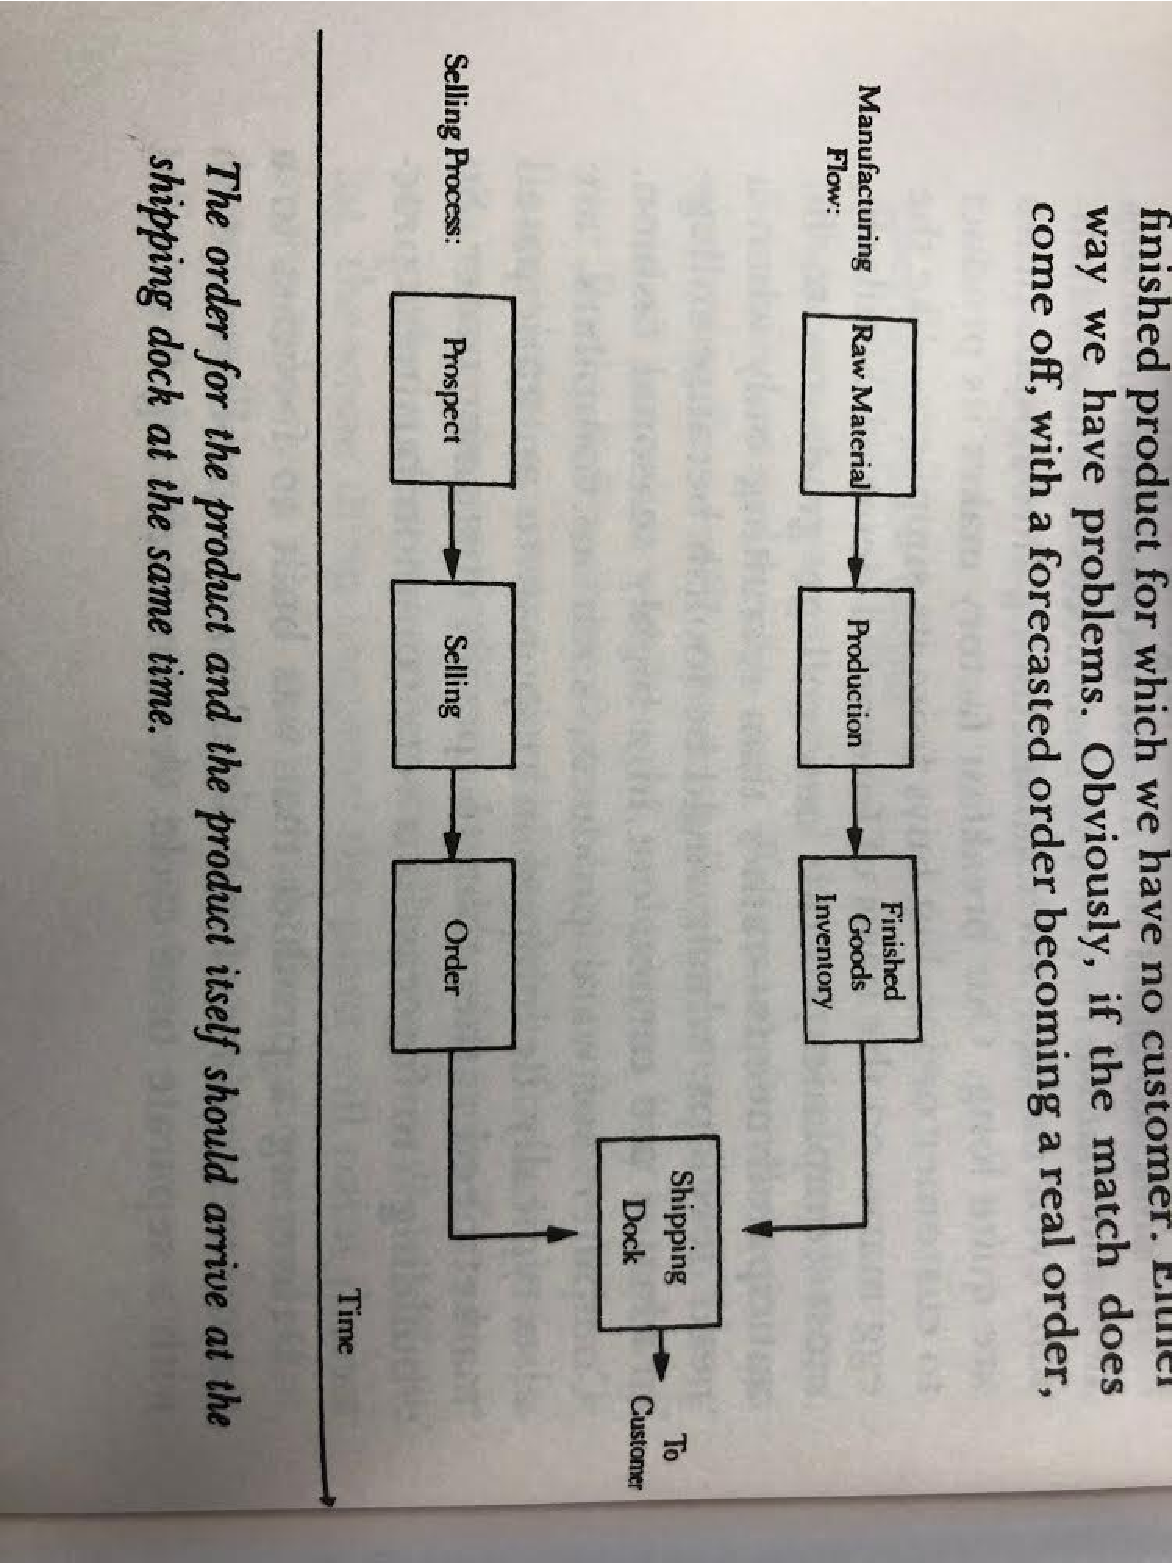
\includegraphics[height=10cm]{deep-parallel.pdf}
  \caption{\label{fig:partitioning} }
\end{figure}

Fail early. Capture failures at the lowest value stage (earlier) that is possible to detect them (needs to be traded off with detection costs). For instance, in candidate recruitment: assess candidate interest early in the pipeline (i.e., during initial phone screens), and if they’re just shopping around then they’re not worth the interview time investment.

Introduce synchronization points as much as possible between parallel flows. Two parallel but dependent features that two teams are working should be incrementalized and should be interacting at as early stages as possible (rather than building two things separately then connect). An example in code development would be to rebase often.

Program slack in volumes of output so that failures downstream can be compensated for. Deadlines for a feature from, say, a customer request, should be made with slack.

Introduce additional quality assurance to take into account the additional risk that the parallel flows incur whenever cheap, continuous tests are amenable (need to trade off w/ quality assurance risk).

\section{Quality Assurance}

\subsection{Gated Tests}

Gated tests, which “hold-the-line” until the completely check out a batch of a product, or take a while to decisively complete, but don’t allow further changes to be made. In software:

\begin{itemize}
\item Diff review
\item Pen test
\item CI is a very cheap gated test
\end{itemize}

\subsection{Sampling-based Tests}

Sampling-based tests probabilistically evaluate for potential failures by taking a look at only parts of the actual total amount of product you’re producing. If they fail then they indicate there’s a broader problem

\begin{itemize}
\item Random selection diff re-review
\item Fuzzy testing and nightly large builds or end-to-end tests, can be coupled with bisection to get gated-level test quality (bisection on commits, for instance).
\end{itemize}

\section{Work simplification}

If you list out the steps for production with fine detail, you can optimize away frequent unnecessary steps.

\begin{enumerate}
\item List out the steps rigorously
\item Set a goal for step reduction
\item Call each step into question
\end{enumerate}

\bibliography{biblio}{}
\bibliographystyle{unsrt}

\end{document}
